\documentclass{article}
\usepackage[utf8x]{inputenc}
\usepackage{ucs}
\usepackage{amsmath} 
\usepackage{amsfonts}
\usepackage{upgreek}
\usepackage[english,russian]{babel}
\usepackage{graphicx}
\usepackage{float}
\usepackage{textcomp}
\usepackage{hyperref}
\usepackage{geometry}
  \geometry{left=2cm}
  \geometry{right=1.5cm}
  \geometry{top=1cm}
  \geometry{bottom=2cm}
\usepackage{tikz}
\usepackage{ccaption}
\usepackage{multicol}

\usepackage{listings}
%\setlength{\columnsep}{1.5cm}
%\setlength{\columnseprule}{0.2pt}


\begin{document}
\pagenumbering{gobble}

\lstset{
  language=C,                % choose the language of the code
  basicstyle=\linespread{1.1}\ttfamily,
  columns=fixed,
  fontadjust=true,
  basewidth=0.5em,
  keywordstyle=\color{blue}\bfseries,
  commentstyle=\color{gray},
  stringstyle=\ttfamily\color{orange!50!black},
  showstringspaces=false,
  %numbers=false,                   % where to put the line-numbers
  numbersep=5pt,
  numberstyle=\tiny\color{black},
  numberfirstline=true,
  stepnumber=1,                   % the step between two line-numbers.        
  numbersep=10pt,                  % how far the line-numbers are from the code
  backgroundcolor=\color{white},  % choose the background color. You must add \usepackage{color}
  showstringspaces=false,         % underline spaces within strings
  captionpos=b,                   % sets the caption-position to bottom
  breaklines=true,                % sets automatic line breaking
  breakatwhitespace=true,         % sets if automatic breaks should only happen at whitespace
  xleftmargin=.2in,
  extendedchars=\true,
  keepspaces = true,
}
\lstset{literate=%
   *{0}{{{\color{red!20!violet}0}}}1
    {1}{{{\color{red!20!violet}1}}}1
    {2}{{{\color{red!20!violet}2}}}1
    {3}{{{\color{red!20!violet}3}}}1
    {4}{{{\color{red!20!violet}4}}}1
    {5}{{{\color{red!20!violet}5}}}1
    {6}{{{\color{red!20!violet}6}}}1
    {7}{{{\color{red!20!violet}7}}}1
    {8}{{{\color{red!20!violet}8}}}1
    {9}{{{\color{red!20!violet}9}}}1
}

\title{Семинар \#3: Массивы. \vspace{-5ex}}\date{}\maketitle
\subsection*{Массивы}
Массивы - это объекты, которые могут хранить внутри себя большое количество других объектов одного типа.
Например, мы можем создать массив, который будет хранить 6 чисел типа \texttt{int} вот так:

\lstset{
  xleftmargin=.3\textwidth, xrightmargin=.2\textwidth
}
\begin{lstlisting}
int a[6] = {4, 8, 15, 16, 23, 42};
\end{lstlisting}

После того, как мы создали массив, мы можем получать доступ к каждому элементу массива по номеру. Номер
элемента массива также называется его индексом. При этом нумерация в массиве начинается с нуля.
\begin{center}
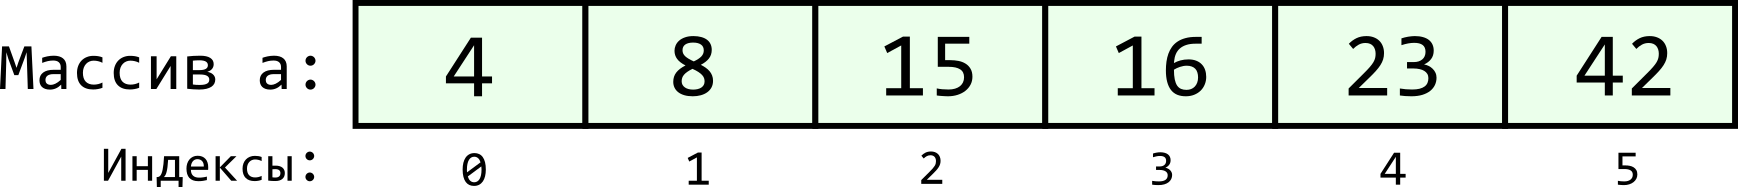
\includegraphics[scale=0.8]{../images/array_indexes.png}
\end{center}
Доступ к элементу по индексу осуществляется через квадратные скобки. Например, если мы хотим поменять в массиве, определённом выше, число 15 на 20 нужно написать:
\begin{lstlisting}
a[2] = 20;
\end{lstlisting}



\subsection*{Подмассивы}
Подмассив - это некоторая последовательная часть массива. В языке C нет никаких специальных средств для работы с подмассивами. Мы будем задавать подмассив в коде как два числа -- индексы граничных элементов. Будем обозначать подмассивом \texttt{a[l, r]} такую часть массива, элементы которого имеют индекс \texttt{i} в диапазоне \\
\texttt{l <= i < r}. Обратите внимание, что мы договорились, что элемент \texttt{a[r]} не входит в подмассив \texttt{a[l, r]}.\\

Например, в подмассив \texttt{[1, 4]} массива \texttt{a} входят элементы \texttt{8, 15, 16}, а элемент \texttt{23} не входит.
\begin{center}
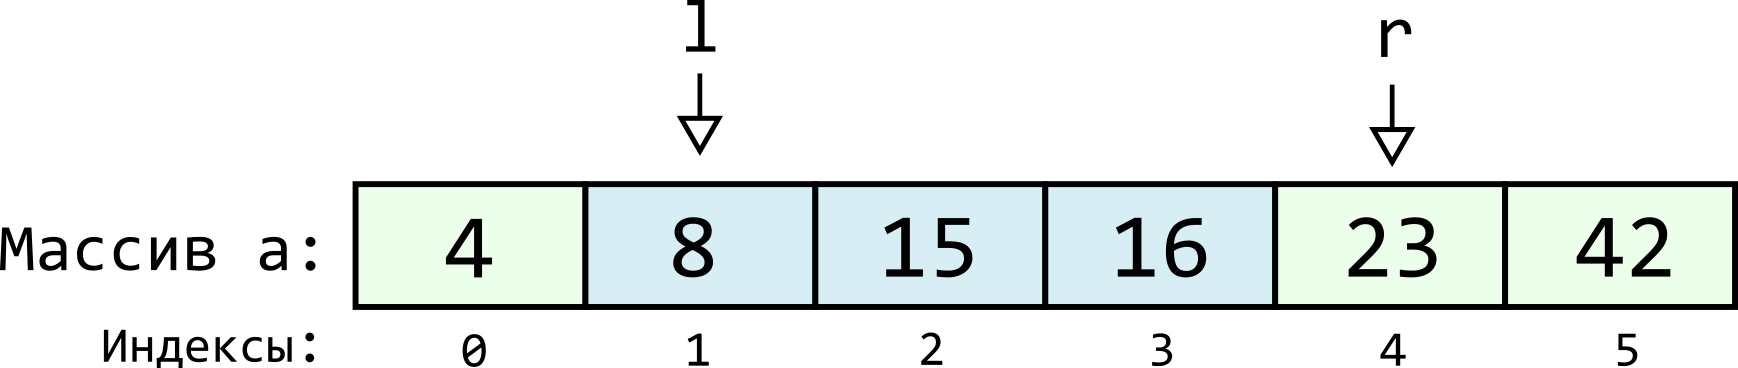
\includegraphics[scale=0.8]{../images/array_slice.png}
\end{center}


\subsection*{Сортировка}
Сортировка -- это упорядочение элементов по возрастанию, убыванию или по какому-то другому критерию.

\subsubsection*{Сортировка выбором} 
Сортировка выбором -- это простейший алгоритм сортировки, который заключается в следующем: \\
Для каждого подмассива \texttt{[j, n]} (где \texttt{j} последовательно меняется от \texttt{0} до \texttt{n - 1}) поменять местами первый и минимальный элементы этого подмассива. 

\subsubsection*{Сортировка пузырьком} 
Сортировка пузырьком -- это простейший алгоритм сортировки, который заключается в следующем: \\
Для каждого подмассива \texttt{[0, n - j]} (где \texttt{j} последовательно меняется от \texttt{0} до \texttt{n - 1}) мы делаем следующую операцию: пробегаем по этому подмассиву и, если соседние элементы стоят неправильно, то меняем их местами.

\end{document}